\section{Program and Design}  

%%%%%%%%%%%%%%%%%%%%%%%%%%%%%%%%%%%%%%%%%%%%%%%%%%%%%%%%%%%%%%%%%%
%%%%%%%%			OBJECTIVES METHODOLOGY AND RESEARCH
%%%%%%%%%%%%%%%%%%%%%%%%%%%%%%%%%%%%%%%%%%%%%%%%%%%%%%%%%%%%%%%%%%

\subsection{Objectives}

\paragraph{}
The objective of this research project is to attempt to answer the overall question of whether a low voltage DC power distribution system could be implemented to power low load devices such as lighting, simple electronics and charging devices. A secondary objective is to relate this project directly to renewable energy generation and in a commercial setting.

\subsection{Methodology}

\paragraph{}
In order to complete this task within a timely manner and ensure all aspects are thoroughly considered and discussed, a clear guideline of tasks musts be followed. Additionally, these tasks will need to specifically address the objectives that the research proposal addresses. As discussed in Section 3, there are five broad questions that are being addressed throughout the two semesters of this thesis. The methodology of the thesis is based around a combination of physical and theoretical testing. A reliance on previous research and design recommendations will be important \cite{Amin2011}. Although research of DC systems has increased, this project will be focusing on an area that has not been sufficiently researched and analysed \cite{Pellis1997}.   

\paragraph{}
The five separate questions are related to the same solution. Initial stages of the project require extensive research on the possibilities and theories behind a purely DC system. Once a strong idea of the possibilities and previous papers were analysed a general analysis of whether or not 48V is the ideal voltage level is secondary. To do this, it will be predominately theoretical with voltage drop calculations over standard cable lengths and areas. Additionally research will be used to back up findings. Software and research will be used to assess the options with solar panels and the best method of implementing them into the solution. 

\paragraph{}
SMART goals will be used to measure the progress. This framework is based off having goals that are specific, measurable, attainable, realistic and timely. These goals are the milestones that are described. By doing so, tasks can be achieved and a regular logbook of activities maintained for process improvements. Spreadsheets and in-built software data storage will be used to record the findings. These findings will be analysed either through additional hand calculations or Matlab. The figure below shows the methodology behind technical design tasks.    

\begin{figure}[H]
\hfill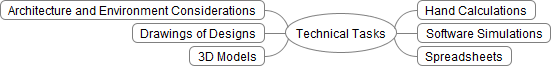
\includegraphics[width = 160mm]{images/Practical_Planning_Rev2}\hspace*{\fill}
\caption{Considerations for a Technical Design Task}
\label{fig:PracProcedure}
\end{figure}     

\subsection{Research Plan}

\paragraph{}
A majority of the project will be through simulations utilising Matlab, PowerCad5, Dialux4.12 and Homer. This is due to power systems electronics being expensive and large scale testing out of the financial scope of this project. Ideally, a full system would be built with Photo-Voltaic cells, battery, controller, DC-DC converters and connections to appliances, however finances will not allow this. Figure 4 below shows a basic PV DC system and the areas requiring consideration. 

\begin{figure}[H]
\hfill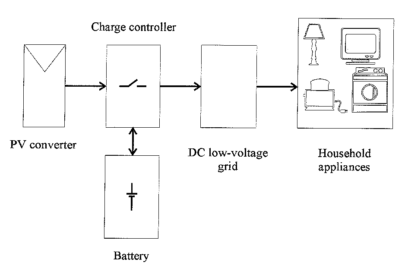
\includegraphics[width = 120mm]{images/DC_Home}\hspace*{\fill}
\caption{Initial Design Consideration for DC Home Power System \cite{Pellis1997}} 
\label{fig:DCHomeSystem}
\end{figure} 

\paragraph{} 
The software will allow for data collection and spreadsheets used to track and assess. The benefit of using spreadsheets and Matlab is that formulas can be input and optimisation simulations run. If simulations are not being used and physical tests are required, a multimeter or computer interfaces will be utilised. If testing cannot be performed or simulated, additional research will be completed to find the closest solution possible. If this method needs to be done, it will explicitly stated in the final report that not all aspects could be physically tested.     

%%%%%%%%%%%%%%%%%%%%%%%%%%%%%%%%%%%%%%%%%%%%%%%%%%%%%%%%%%%%%%%%%%
%%%%%%%%			FINANCE
%%%%%%%%%%%%%%%%%%%%%%%%%%%%%%%%%%%%%%%%%%%%%%%%%%%%%%%%%%%%%%%%%%

\subsection{Resources and Funding}

\paragraph{}
The design and construction of this project would require a substantial amount of resources. Due to this, computer assisted design (CAD) programs will be used as the main design calculation feasibility analysis mechanism. The University facilitating this research project will allocate \$50 for each student through purchase order applications. This value will be taken into consideration when designing possible testing mechanisms or models for the presentation. 

%%%%%%%%%%%%%%%%%%%%%%%%%%%%%%%%%%%%%%%%%%%%%%%%%%%%%%%%%%%%%%%%%%
%%%%%%%%			TEAM
%%%%%%%%%%%%%%%%%%%%%%%%%%%%%%%%%%%%%%%%%%%%%%%%%%%%%%%%%%%%%%%%%%

\subsection{Project Team}

\paragraph{}
As previously stated, this project is being solely undertaken, however there are three students undertaking topics that are interrelated. In addition to my task focusing on low voltage DC systems in larger applications, the other two students are analysing sub issues in the same broad category. There will be discussions between the three students on relevant articles, journals and standards that each person finds.

%%%%%%%%%%%%%%%%%%%%%%%%%%%%%%%%%%%%%%%%%%%%%%%%%%%%%%%%%%%%%%%%%%
%%%%%%%%			TIMELINE
%%%%%%%%%%%%%%%%%%%%%%%%%%%%%%%%%%%%%%%%%%%%%%%%%%%%%%%%%%%%%%%%%%
\newpage
\subsection{Project Timeline}

\paragraph{}
This project will be predominately based on two major resources; software availability and personal time. Software will be available at all times due to the University providing paid software packages and myself already having installed free ones. Personal time will be the major difficulty as it will be balanced between other University classes, part-time work, and personal responsibilities.   

\paragraph{}
The tasks were be split into days and University weeks. It was ensured to include the holidays that University allows. This project does not simply end upon the completion of this semester. BEB801 is concluded on November 4th at the end of Week 14, however BEB802 is the subject allocation to complete the second half of this project. The task table will allocate SMART milestones. Additionally, the benefits of completing the subjects during this period is that there is the additional time from summer holidays to account for.

\paragraph{}
Table \ref{table:milestones_1} on the following page shows the milestones of this project. The University assigned submissions are represented as bold text. The four major deliverables for the first half of this project are the library assessment, project proposal, oral presentation and progress report. These four deliverables are what have outlined how the remaining tasks have been created and the time periods allowed for. Earlier due dates are set to allow for editing or possible difficulties to occur without major repercussions. 

\paragraph{}
The assessed deliverables for Semester 2 are similar to the first. The major difference predicted is that the task should be very well understood by the beginning of semester. By having this advantage as well as the additional time during summer break, it allows for a very strong foundation for the final design. This is why the non-assessed milestones are predominately finalisation throughout the entire semester. The summer break will be utilised to reduce the required work during the University period. 

% Table of Tasks
\begin{table}[H]
\centering
\begin{tabular}{||c c||} 
 \hline
 \multicolumn{2}{|c|}{\textbf{Initial Project Timeline}} \\ [0.5ex] 
 \hline\hline
 \textbf{Milestone} & \textbf{Deadline} \\ 
 \hline\hline
 Project Definition & Week 3 \\ 
 \textbf{Library Assessment} & \textbf{Week 4} \\
 Initial Research Phase & Week 6 \\
 \textbf{Project Proposal} & \textbf{Week 7} \\
 Initial Design Phase & Week 9 \\
 Initial Prototype Design Finalised & Week 11 \\
 Initial 3D Modelling for Presentation & Week 12 \\
  \textbf{Initial Oral Presentation} & \textbf{Week 14} \\ 
 \textbf{Written Report} & \textbf{Week 14} \\ 
 Implement Feedback From Report & Summer Break \\
 Complete Research Shortcomings & Summer Break \\
 Complete Further Technical Calculations & Summer Break \\
 Initial Finance Analysis & Week 2 \\
 Design Simulations & Week 6 \\
 \textbf{Progress Report} & \textbf{Week 7} \\
 Finalised Design & Week 10 \\
 Finalised Simulations \& 3D Modelling & Week 11 \\
 Finalised Financial Analysis & Week 12 \\
 \textbf{Final Presentation} & \textbf{Week 14} \\
 \textbf{Final Report} & \textbf{Week 14} \\ [1ex] 
 \hline
\end{tabular}
\caption{Initial Project Timeline}
\label{table:milestones_1}
\end{table}    

\subsection{First Stage Analysis of Timeline}

\paragraph{}
This section outlines the initial analysis of the originally projected timeline. Table \ref{table:milestones_2} above will be replicated with additional analysis of whether or not milestones have been reached and if they were on time. Additionally, if aspects of the project has changed and the timeline needs to be re approached, this will be done.  

% Table of Tasks
\begin{table}[H]
\centering
\begin{tabular}{||p{5cm} c c||} 
 \hline
 \multicolumn{3}{|c|}{\textbf{Initial Project Timeline Analysis}} \\ \hline\hline
 \textbf{Milestone} & \textbf{Original Deadline} & \textbf{Actual Completion} \\ [0.5ex] 
 \hline\hline
 Project Definition & Week 3 & Week 3\\ 
 \textbf{Library Assessment} & \textbf{Week 4} & Week 4\\
 Initial Research Phase & Week 6 & Week 6\\
 \textbf{Project Proposal} & \textbf{Week 7} & Week 7\\
 Initial Design Phase & Week 9 & Week 10\\
 Initial Prototype Design Finalised & Week 11 & NA\\
 Initial 3D Modelling for Presentation & Week 12 & Week 11\\ 
 \textbf{Initial Oral Presentation} & \textbf{Week 14} & Week 14\\
 \textbf{Written Report} & \textbf{Week 14} & Week 14\\ 
 Implement Feedback From Report & Summer Break & TBC \\
 Complete Research Shortcomings & Summer Break & TBC \\
 Complete Further Technical Calculations & Summer Break & TBC \\
 Initial Finance Analysis & Week 2 & TBC \\
 Design Simulations & Week 6 & TBC \\ 
 \textbf{Progress Report} & \textbf{Week 7} & TBC \\
 Finalised Design & Week 10 & TBC \\
 Finalised Simulations \& 3D Modelling & Week 11 & TBC \\
 Finalised Financial Analysis & Week 12 & TBC \\ 
 \textbf{Final Presentation} & \textbf{Week 14} & TBC\\
 \textbf{Final Report} & \textbf{Week 14} & TBC\\ [1ex] 
 \hline
\end{tabular}
\caption{Initial Project Timeline Analysis}
\label{table:milestones_2}
\end{table}      

\paragraph{}
The first major change from the first revised timeline is that the initial prototype design is now NA. The reasoning behind this is due to the slight change in planning for the project since the initial proposal submission. Since creation of the timeline, the scope has been re-approached and instead of ensuring a prototype converter is built by the end of the project, the questions have been refocused and more specific simulations will be reached. The design of a converter is a secondary if time allows. 

\paragraph{}
The next milestone was initial 3D modelling of the building design for the presentation. This was completed but not as extensively as I would have liked. The access to Queensland of University's power consumption, floorplans, lighting plans and photovoltaic system configuration. This data was only made available in Week 11 which was later than possibly to fully utilise it before the presentation of progress. Due to this, the summer break tasks will be required to be extended to make up for the loss of time during Semester 1. This data will be used to finalise a floorplan that can be analysed and the concept of a low voltage DC distribution system proven feasibly or not.  

% Table of Tasks
\begin{table}[H]
\centering
\begin{tabular}{||c c||} 
 \hline
 \multicolumn{2}{|c|}{\textbf{Revised Timeline for Remaining Tasks}} \\ \hline\hline
 \textbf{Milestone} & \textbf{Deadline}\\ [0.5ex] 
 \hline\hline
 Implement Feedback From Report & Summer Break  \\
 Complete Research Shortcomings & Summer Break  \\
 Finalise Floorplan and Load Demand & Summer Break  \\
 Complete Further Technical Calculations & Summer Break  \\
 Initial Product Decisions & Week 3  \\
 Initial Finance Analysis & Week 4  \\
 Design Simulations & Week 6  \\ 
 \textbf{Progress Report} & \textbf{Week 7}  \\
 Finalised Design & Week 10  \\
 Finalised Simulations \& 3D Modelling & Week 11  \\
 Finalised Financial Analysis & Week 12  \\ 
 \textbf{Final Presentation} & \textbf{Week 14} \\
 \textbf{Final Report} & \textbf{Week 14} \\ [1ex] 
 \hline
\end{tabular}
\caption{Revised Timeline for Milestones}
\label{table:milestones_3}
\end{table} 
